\documentclass[12pt]{article}
\usepackage[top=30truemm, bottom=30truemm]{geometry}

%draftの場合[dvipdfmx]を[draft]
\usepackage[dvipdfmx]{graphicx}
\usepackage{newtxtext}
\usepackage{layout}
\usepackage{lineno}

\usepackage{url}
\usepackage{float}
\usepackage{array}
\usepackage{subcaption}
\usepackage{setspace} 
\setstretch{2}
\usepackage{makeidx}
%bibliographyに必要なパッケージ natbibzip内
%https://ja.sharelatex.com/learn/Bibliography_management_with_natbib
\usepackage{natbib}
\usepackage{lscape}
\usepackage[dvipdfmx]{color}
\usepackage[dvipdfmx]{hyperref}
\usepackage{pxjahyper} %%hyperref読み込みの直後に
\usepackage[toc,title,page]{appendix}

\begin{document}
\linenumbers
\begin{abstract}
mac book proで更新
こんどはmac proで更新 できたかな?
Studying the physics of experiments using common materials to simulate geological processes frequently provides novel ideas and insight that can be applied to natural phenomena.
In this study, a physical system of a laboratory experiment that is assumed to be mathematically equivalent to volcanic eruption systems and its behaviors and physical processes are investigated.
This study aims to obtain through a laboratory experiment such new insight and ideas that it would be difficult to find directly from field observation and mathematical modeling of volcanic systems.

In this study, the physics of a pipe-chamber eruption experiment was investigated. 
This experiment was inspired by a sugar syrup eruption experiment conducted as an exhibition during an institute open house. 
The experimental system comprised a vertical pipe connected to a gas chamber where a constant gas flux was maintained in the gas chamber and the gas-liquid flow in the pipe.

First, pressure changes in the chamber were investigated. Sawtooth wave-like pressure changes (STW) were observed during the constant gas supply. Similar waveforms have been observed as geodetic signals that are associated with repetitive explosive eruptions and Dome-building eruptions.
Volcanic oscillations have been explained by flow-induced oscillation models that include a coupling between elastic capacitance and variable flow resistance.
Behaviors of these systems have not been studied by laboratory experiments. 
It was shown that the experimental system of this study was mathematically similar to the existing volcanic oscillation models.
The chamber pressure changes and flows in the pipe in the experiment were comparable with magma chamber pressure changes and conduit flows in volcanic systems, regardless of differences in specific scales and flow structures.
In the experiment, periodicity spontaneously varied in either non-periodic, bimodal or trimodal manners, even if the given experimental parameters such as the pipe-chamber geometry and gas influx were constant.
These had not been expected from existing models of volcanic systems. 
Finding such new phenomena is a significance of the lumped parameter model experiment of volcanic systems.
As a result of the flow image analysis, it was concluded that the spontaneous periodicity fluctuations were caused by variations of flow structure in the pipe due to past gas emissions.
I inferred that, in the actual volcanic systems, fall-back of ejected materials, dike collapse, or different depth of magma head could disturb periodicity of an eruption.

Second, acoustic waves were measured at the top of the pipe in association with the chamber pressure oscillations and gas emissions.
The acoustic waveforms were disturbed preceding that the flow structure in the pipe and the chamber pressure periodicity were disturbed.
In general, the acoustic waveforms with the sawtooth wave-like pressure changes in the chamber had two characteristic frequency peaks. The peak frequencies were explained by two different resonance models.
It was shown that the amplitude of the lower frequency band in the acoustic wave had good correlation with the sawtooth wave amplitude in the chamber.
Although the mechanisms of acoustic wave generation in this experiment and those in volcanic systems have not sufficiently linked, this experimental results suggested a possibility to find a correlation between a particular component of infrasound and ground deformation observed in actual volcanic eruptions.

Finally, relationships among ground deformation, infrasound, and video records during 2015 Sakurajima volcanic activity were investigated.
The recurrence interval of sawtooth wave-like ground deformation was by far disturbed compared to the experimental results. It was not successful in finding a relation between successive events that was comparable with the experimental system.
The main finding was that the correlation between the sawtooth wave amplitude of ground deformation and the cumulative energies of small infrasound signals during the individual ash eruption events. It was suggested that the infrasound energy would be a useful parameter for monitoring eruptive volcanic activity.
                
In this study, I have not completed updating volcanic models based on insights and ideas obtained from experiments.
On the other hand, showing the mathematical similarity between the experiment and volcanic eruption systems, finding disturbed periodicity and the correlation between a particular resonance model of infrasound and chamber pressure were important results. 
They were unique outcomes of a model experiment of volcanic systems. 
The obtained relationship between infrasound and ground deformation at Sakurajima was found as a result of reviewing and analyzing the observational data applying insights from the laboratory experiment.
Based on the above results, this experimental system may provide a useful tool for understanding volcanic eruption system.
\end{abstract} 



\newpage
\cleardoublepage


\section{Introduction}\label{ACOintro}
実験では, チャンバーの圧力変動を計測するとともに, パイプ上端において空気振動も計測している. 

ここにも変更を加えると?

火山活動にともなっても, 主に 20 Hz 以下の帯域にパワーを持つ空気振動 (以下, 空振) が観測される. 
空振観測は, 天候不良や夜間, 離島での噴火といった監視カメラ等を備えた観測点がない場合でも, 噴火発生とその方向を検知することができるため, 防災上の観点から重要な物理観測量の一つである.
また, 空振はそれぞれの火山活動において, 様々な特徴的周波数・波形を持っており, 発生メカニズムを考えることによって, 噴火機構の理解や, 噴出量・噴出率といった噴火パラメータを推定できることが期待される. 

本章では, 実験で計測した空気振動を解析して, 発生メカニズムを特定し, 同時に記録したチャンバー圧力や流動様式との対応関係を明らかにすることを目的とする. 実験の空気振動に関しては, 特に周波数構造に着目した上で, メカニズムを検討する. また, 空気振動とチャンバー圧力の対応関係を踏まえて, \S \ref{FLD} では火山活動において観測される空振と, 地盤変動の関係性を検討する.



\subsection{Laboratory experiments}\label{AcoinEx}
\cite{Vidal2006a}では, 円筒状のCavity上部に張った石けん膜が, Cavity内部の過剰圧によって割れる際の空気振動を計測した. 
この実験は, 大気泡が火道浅部で破裂すると考えられているストロンボリ式噴火 \citep{Chouet1974, BLACKBURN1976, Vergniolle1996c}での空振発生プロセスを再現していると考えられている \citep{Vidal2010a, Gerst2013a}. 
この実験において, 発生する空気振動の周波数構造は, Cavity内の定在波, すなわち, 閉管の気柱共鳴で説明できる. 一方で, 破裂後, 管の外で計測した空気振動の振幅は, 破裂直前のCavity内の過剰圧には相関せず, 膜の破裂過程に大きく影響される. すなわち, キャップの破裂・破壊をともなうような噴火においても, 空振の振幅はキャップの破裂・破壊過程に影響を受ける可能性が示唆される \citep{Vidal2010a}. \cite{Sanchez2014}では, 石けん膜の代わりに, Elastic membraneを用いて破裂速度を制御した実験を行った. この結果, やはり特徴的な周波数は閉管気柱共鳴で説明できる. また, 膜の破裂速度を制御すれば, 破裂前の過剰圧が小さい (この実験では 24 kPa以下) 時に, 破裂前過剰圧と破裂時の空気振動振幅が線形な関係にあることを示した. 

流体内を上昇し, 表面で破裂する気泡によって発生する空気振動も, 室内実験によって調べられている.
\cite{James2004}では, 鉛直パイプ内に満たされたニュートン流体中のガススラグの上昇と破裂過程における空気振動を計測した. 連続的なガススラグの上昇と破裂の際に計測された空気振動の特徴的な周波数は閉管の気柱共鳴で説明できる. 
\cite{Spiel1992}では, 気泡サイズよりも十分に大きな水槽中を上昇する気泡の破裂によって生じる空気振動を計測した. 空気振動の特徴的周波数は気泡破裂時の気泡体積と, 気泡サイズに対して小さい開口面積に由来するヘルムホルツ共鳴であると推定している.
\cite{Divoux2008}では, 非ニュートン流体中を上昇する気泡の破裂にともなう空気振動を計測した. 空気振動の特徴的な周波数は, カスプ状に尖った気泡の形状に依存する共鳴音であると推定している.


\subsection{Observation}\label{AcoinObs}

ストロンボリ式噴火では, 低粘性マグマ中を大気泡が上昇し, 表面で破裂すると考えられている. 大気泡の破裂にともない, 継続時間が数秒程度のパルス状空振が発生する. 
%マイクの特性が議論されている論文を見つけることができず, 一旦波形の議論はそのまま
\cite{Vergniolle1996b} では1992年, ストロンボリ島 (イタリア) において空振観測を行った. この観測では Br\"uel-Kj\ae r社製マイク (Type 4155, 1 Hz - 70 kHz, Type 4165, 4 Hz - 20 kHz) を用いて, 3点の観測点 (東火口から約 250 m地点に 2点, 約 370 m地点に 1点) で, 1 kHzサンプリングで空振を記録した. 
この時期のストロンボリは, 西火口ではマグマを目視でき, 泡の破裂が確認できる. 一方で, 東火口の活動は比較的穏やかであった. 
東火口で発生した爆発の際に観測した空振にともなって, Fig. \ref{Verg19961fig1}aのような波形を観測し, 主要相では約 10 Hz にピークを持つ (Fig. \ref{Verg19961fig1}c). この波形を説明するメカニズムとして, \cite{Vergniolle1996c} では, 気泡破裂前の, 気泡膜振動が提案されている. 
しかし一方で, 近年のレーダー観測を用いた大気泡膨張過程における気泡膜移動速度の直接観測   \citep{Gerst2013a} によれば, 膜の振動は計測されず, 大気泡は空振波形の希薄相が始まる前に破裂しており, 特徴的周波数は膜の破裂後, 表面に取り残された空洞部分の共鳴であると推定している (Fig. \ref{gerst2013f14}).


ブルカノ式噴火は島弧の安山岩質火山でしばしば発生し, 単発的・間欠的に爆発が起こる噴火である. \cite{Iguchi2008}では, 地震と地盤変動観測の解析から, 火道浅部のプラグが破壊されることによって噴火が発生していると推定している.
主にブルカノ式噴火が間欠的に発生している桜島において, 2011年7月から12月にかけて, 昭和火口の噴火を対象とした空振観測が実施され, 噴煙を上げる噴火の空振が, ふたつの特徴的ピーク周波数 (0.2 - 0.5 Hz と1 - 2 Hz) を持つことが報告されている (Fig. \ref{yokoo2012bof4}) \citep{yokoo2012bo}. この観測では白山工業社製マイク (SI102) を用いて, 昭和火口から約 3.3 km東にある黒神観測点において, 200 Hzサンプリングで, 9台のマイクを用いたアレイ観測を行った.
三次元噴煙計算 \citep{Suzuki2005} によって, 噴出率 10$^6$ kg/s, 噴出速度 133.67 m/s, 温度 1273.15 K, 火口直径 20.37 m の時の噴煙を再現すると, 0.3 - 0.6 Hzあたりにパワーが集中し, 1 - 2 Hz付近のシグナルは含まれない. 
一方で, 実際の観測値においては, 1 - 2 Hzのシグナルは噴火発生の有無と関係なく観測される. 従って, \cite{yokoo2012bo} では, 0.2 - 0.5 Hzのシグナルは噴煙から放射されており, 1 - 2 Hzの周波数帯のシグナルは, 火口や火道部分がガスや噴煙の通り道となることで固有振動数が強められるのではないかと考えられている. 

継続時間が長い, 微動型の空振も報告されているが, 本実験では, チャンバー圧力振動にともなって, パルス的な空気振動が発生しているため, 微動型空振の先行研究は簡潔にまとめる. 
%詳細についてはAppendix (\S \ref{appeaco}) にまとめる.

チリのビジャリカ火山では, 溶岩湖内マグマの対流と, 表面での気泡破裂が発生している時期に, 0.77 Hz付近にピークを持つモノトニックな空振が報告されている \citep{Ripepe2010b, Goto2011}. 
\cite{Ripepe2010b}では, 計測されるモノトニックな周波数ピークは気液二相流の重力的な不安定による火口湖表面の振動に起因すると推定した. %Ripepe2010 p4
一方で, \cite{Goto2011}で撮影したビデオ映像によれば, 火口湖表面での対流や脱ガス活動と, 空振記録との間に明瞭な関係が見られなかったことから, 特徴的周波数は空洞状の火口内気体の体積振動, すなわちヘルムホルツ共鳴であると考えられている. %Goto2011 p.3
このような空洞状の火口内のヘルムホルツ共鳴と考えられる空振は, キラウェア火山 (ハワイ), ハレマウマウ火口における連続的な脱ガス活動の際にも報告されている \cite{Fee2010c}. 
この活動で観測された空振には, もう一つ特徴的なピークがあり, 空洞状の火口内の定在波であると推定されている (Fig. \ref{fee2010bfig3}). 

セントへレンズ山 (アメリカ)では, 2005年3月に, 最大高度が 9 km程度の噴煙柱を形成する噴火の際に, 0.2 Hz付近に周波数ピークを持つような空振を観測した (Fig. \ref{matoza2009f2}). 
%この観測では, MB2000微気圧計 (0.01-17 Hzで平坦な特性)を用いて, 火口から13 km 北西のColdwaterという観測点で, 40 Hzサンプリングで4点空振アレイ (100 m間隔) 観測を行った. 
この周波数構造は, ジェットノイズの周波数構造と相似的であり, 自己相似的なノイズ (Large-scale turbulence) 生成メカニズムの存在が示唆される \citep{Matoza2009a}.

エクアドルのトゥングラワ火山 \citep{Fee2010} では, 2006年7月14-15日 (UTC) の噴火で, 火口直上に噴煙柱を形成する継続的なジェット噴出の際に, 0.25 Hz付近と 1 Hz付近に幅の広い2つのピークを持ち, その間にノッチを持つような周波数構造を持つ空振を記録した (Fig. \ref{fee2010afig9}点線). 一方で, 7月15日 2:45 (UTC) ごろに発生した Pyrocclastic density current (PDC) にともなって記録された空振では, 0.25 Hzのみにピークを持つ周波数構造であった. 1 Hz付近のピークは, 噴煙柱を形成するような噴火において見られる特徴的ピークであることから, 自己相似的なノイズ (Large-scale turbulence) 生成メカニズムの存在が示唆される \citep{Matoza2009a}. また, 0.25 Hzのピークは, PDC 発生時においても見られたことから, 流れと火口壁との相互作用に起因すると考えられている.
%噴煙柱を形成するような噴火では 1 Hzのピークが見えるため, 1 Hzのピークはジェットノイズに関係し, 0.25 Hzのピーク固体粒子間の相互作用に由来するのではないかと考えられているが \citep{Matoza2009a}, 定量的な議論はなされていない.


基本周波数と, その倍音成分を持つハーモニックな微動型空振も多くの火山で報告されている. サンガイ山 (Sangay, エクアドル)では, 1998年4月の観測で, Chugging発生時に基本周波数が約1 Hzのハーモニックな微動型空振を計測している \citep{Johnson2000}. Chugging発生と同期したハーモニックな微動型空振は, アレナル山 (Arenal, コスタリカ, 1997年) \citep{Hagerty2000}, カリムスキー山(Karymsky, ロシア, 1997-98年) \citep{Johnson2000}, レベンタドル山 (Reventador, エクアドル, 2005年) \citep{Lees2008}, 桜島 (2017年) \citep{sakai1996, iguchi2018} でも報告されている.


\clearpage
\subsubsection{空振記録を基にした噴火パラメータの推定}\label{AcointPara}

火山活動にともなう空振記録の解析と, そのほかの物理観測量とを用いることで, 噴火の物理過程や, パラメータを推定する試みがなされている. 

爆発的噴火にともなうパルス状の空振に関しては, 空振のソースが単純なモノポールソースであると仮定し \citep{Lighthill1978}, 積算体積を推定する手法が提案されている \citep{Johnson2003}. この手法を用いて, 空振から見積もった積算体積と, そのほかの観測量とか比較されている.

火山灰の放出が少なく, ガスの放出が主であるような, Gas-rich な火山活動において, \cite{Dalton2010}では, モノポールソースを仮定して空振波形を二回積分して推定した噴出体積と, UVカメラを用いたSO$_2$噴出体積との関係を調べ, おおむね比例関係にあることを示した.
また, 多くの火山灰放出をともなう Ash-richな火山活動, とくに爆発的噴火に関して, \cite{Fee2017a}では, 桜島の爆発空振から推定した噴出量, 火山灰降下量, ガス観測から推定した噴出量とを比較した. この結果, 空振から推定した噴出量と, 火山灰の堆積分布から推定した噴出量とは, 一桁程度のばらつきをもって比例関係があると主張している.
\cite{Yamada2018b}では, 空振波形の積分から推定した噴出体積 ($V_{inf}$)と, 時定数の短い噴火にともなう噴煙をサーマルに近似することで推定した噴煙体積 ($V_{b}$) の関係を調べた. この結果, $V_{b}/V_{inf}=16$という関係を得た. 空振から推定した体積は, 爆発の初動段階で火口付近で押しのけられた体積を反映していると考えている. 

しかし一方で, Gas-rich, Ash-richな噴火それぞれに, 単純にモノポールソースを仮定して良いかは自明ではない. \cite{DelleDonne2016} では, イタリア, ストロンボリ火山における空振記録に対して, いくつかの手法を用いて爆発時のガス放出量を推定し, Thermal cameraを用いた熱エネルギーと, カメラを用いたSO$_2$ガス放出量と比較している. 
空振の主要相を用いた推定ガス放出量と熱エネルギーは, Gas-richなイベントでは相関が良いが, Ash-richで継続時間が長いイベントでは相関が悪い. 一方で, 空振の後続波まで考慮する手法を用いた空振ガス放出推定量は, Gas-richなイベントもAsh-richなイベントも熱エネルギーとよく相関している (Fig. \ref{DelleDonne2016fig3}). 


\cite{Ichihara2016a}では, 新燃岳 2011年噴火の際に観測された3回のサブプリニー式イベントにおいて, 地盤変動から推定した噴出率 ($\dot{V}_m$) と, 地震・空振パワー (SET, AET) の関係を調べた. この結果, 準定常的サブプリニーイベント発生時には, $\dot{V}_m$は SET とも AET とも, 線形関係にあることを示し, 定常的な噴火の際の空振が, 破砕面での連続的な爆発によって励起されていると推定している. この結果からは, ある特定のイベントにおける空振に着目すれば, 空振と噴出率・量の対応関係を見出すことができる可能性が示唆される.




\clearpage \newpage
\subsection{実験結果}\label{ACOresult}
実験装置及び実験手法は \S \ref{PRE} で行なった実験と同じである. 本章では液スラグ膜の破裂によって発生し, パイプ上端のマイクで捉えた空気振動に着目する. そして, 空気振動と, 前章で議論したチャンバー圧力振動との関係に主眼を置く.  

\subsubsection{計測された空気振動の概要}
Unimodal STW が発生している時 ($Q_\mathrm{in}=$ 0.6 cm$^3$/s, $V_\mathrm{c}=$ 122 cm$^3$) のチャンバー圧力と空振記録の時間変化をFig. \ref{MonoPAtime}に示す. 
振幅の大きな (> 10 Pa) 空気振動は, STWの急激な圧力減少と同期している.
空気振動の代表的な波形とスペクトルを Fig. \ref{Monowaveform}に示す. 実験において, 圧力急減少の有無を問わずに, 空気振動パルスの最大振幅が 1 Pa以上になるようなパルスをトリガし, 縦軸が周波数, 横軸がパルスイベントになるように並べた図を Fig. \ref{Monopspec}に示す. イベントは, 20 Hz付近のピークの大きさでソートしてある.  この結果によれば, 低周波帯 ($\sim$ 20 Hz) にピークを持つ波形は, 230 - 270 Hz付近にもピークを持つ. 一方で, 低周波帯にピークを持たないパルスは, 180 - 200 Hz付近に明瞭なピークをもち, 270 Hz付近に小さいピークを持つ. この実験条件で発生する空振のうち, 半数程度は低周波帯にピークを持たない空振であった. 以下, 低周波帯 (< 50 Hz) と高周波帯 (> 150 Hz) にピークを持つパルスを低周波パルス, 高周波帯 (> 150 Hz) のみにピークを持つパルスを高周波パルスと呼ぶ. 

Small fluctuation 発生時, すなわち, 連続的なスラグ流が計測される際のチャンバー圧力と空振記録を Fig. \ref{FlctPAtime} に示す.  STW発生時と比較して, チャンバー圧力変動との対応は不明瞭であるが, 概ね緩やかな圧力減少と空気振動の発生が対応している. 代表的な波形を Fig. \ref{Flctwaveform} に示す. パルスの振幅はSTW発生時と比べて小さく, 低周波帯にピークがみられない. Fig. \ref{Flctpspec} に Fig. \ref{Monopspec}と対応した図を示す. この実験条件では, 180 - 200 Hz程度に基本周波数を持つ振動が発生している. 波形及び周波数ピークの特徴から, STW発生時の高周波パルス (Fig. \ref{Monowaveform}a-c) と同じ性質を持つ. 

Disturbed STW について, チャンバー圧力と空振記録の時間変化を Fig. \ref{DistPAtime}に示す. Disturbed STWにおいても, 基本的に大きい振幅の空気振動は圧力の急減少にともなって発生している. 代表的な波形を Fig. \ref{Distwaveform} に示す. Unimodal STWと同様に低周波パルスと高周波パルスが発生している. また, 低周波パルスは, Unimodal STWで発生する空気振動波形と比べてバリエーションがある. Fig. \ref{Distpspec} によれば, 高周波パルスは全体の1割程度である. 


実験パラメータと, 空振の振幅の関係をFig. \ref{QVA} に示す. 実験パラメータの $Q_\mathrm{in}$, $V_\mathrm{c}$と, 空気振動パルスの平均振幅は明瞭な相関が見られない. 

Fig. \ref{PAPCall}a, bに, それぞれの圧力変動パターンにおいて発生する空気振動パルスに関して, 生波形の振幅と, 高周波帯 (50 Hz >), 低周波帯 (50 Hz <) にバンドパスフィルターをかけた場合の振幅との関係を示す. 計測した空気振動パルスの生波形振幅は, 高周波帯のシグナルの振幅を表しており (Fig. \ref{PAPCall}b), 生波形振幅と低周波帯振幅は全く関係がない (Fig. \ref{PAPCall}a). 

\clearpage
\begin{figure}[H]
\begin{center}
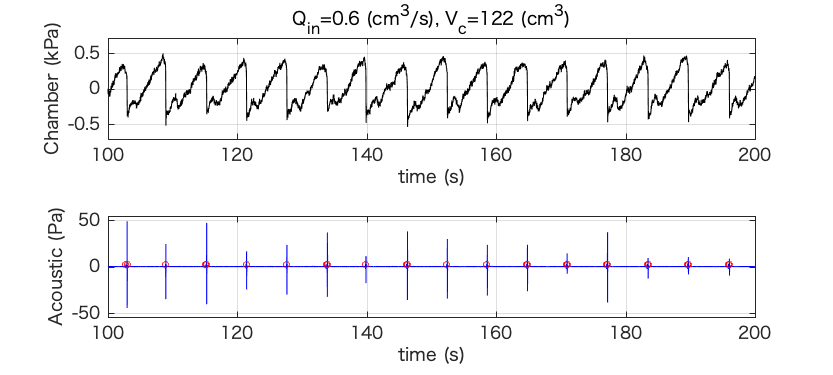
\includegraphics[scale=1] {MonoPAtime.png} 
\caption[チャンバー圧力と空気振動: Unimodal STW]
{チャンバー圧力と空気振動 (Unimodal STW): 上段 チャンバー圧力波形, 下段: 空気振動波形, 下段の赤○マーカーは, 急激な圧力減少がトリガされた時間.}
\label{MonoPAtime}
\end{center}
\end{figure} 

\begin{figure}[H]
\begin{center}
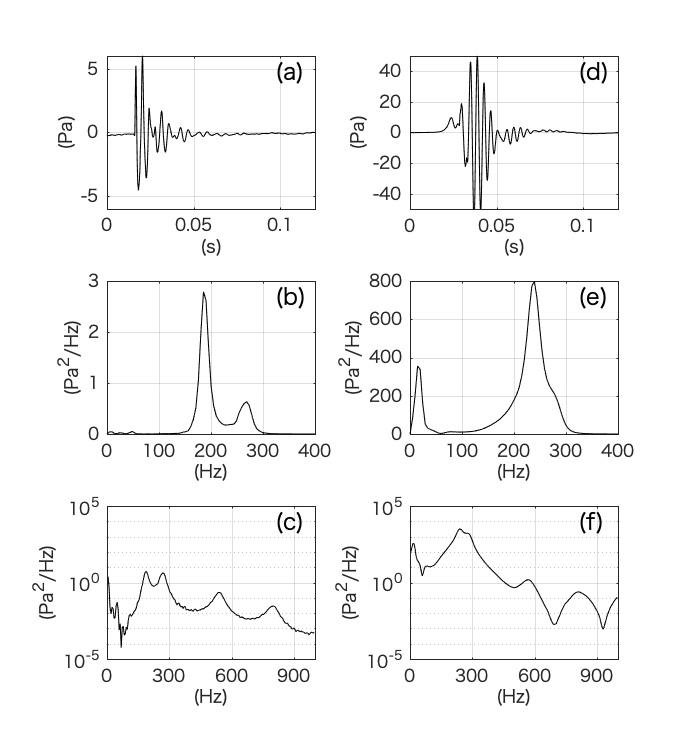
\includegraphics[scale=1] {Monowaveform.png} 
\caption[代表的波形と周波数構造: Unimodal STW]
{代表的波形と周波数構造: Unimodal STW. (a) の波形は高周波成分しか持たない高周波パルス (b, c). (d) の波形は高周波成分と低周波成分を持つ低周波パルス (e, f).}
\label{Monowaveform}
\end{center}
\end{figure}

\begin{figure}[H]
\begin{center}
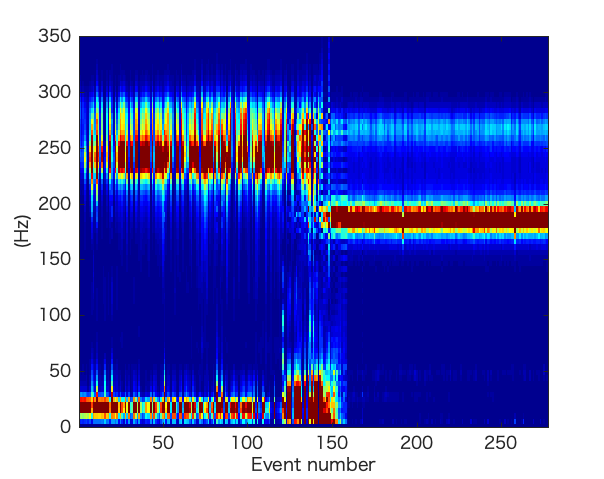
\includegraphics[scale=1] {Monopspec.png} 
\caption[イベント毎のスペクトル構造: Unimodal STW]
{イベント毎のスペクトル構造 (Unimodal STW): 圧力急減少の有無を問わずに, 空気振動パルスの最大振幅が 1 Pa以上になるようなパルスをトリガした. 縦軸は周波数, 横軸はパルスイベントに並べてあり, 20 Hz付近のピークの大きさでソート.}
\label{Monopspec}
\end{center}
\end{figure} 

\begin{figure}[H]
\begin{center}
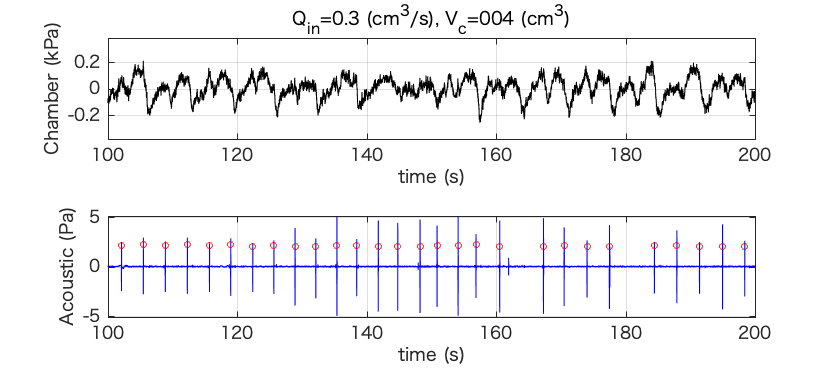
\includegraphics[scale=1] {FlctPAtime.png} 
\caption[チャンバー圧力と空気振動: Small fluctuation]
{チャンバー圧力と空気振動: Small fluctuation, Fig. \ref{MonoPAtime}のキャプションを参照}
\label{FlctPAtime}
\end{center}
\end{figure} 

\begin{figure}[H]
\begin{center}
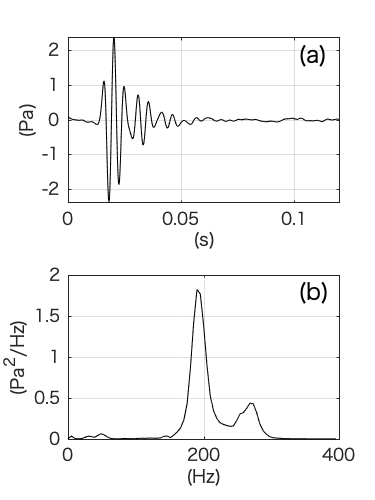
\includegraphics[scale=1] {Flctwaveform.png} 
\caption[代表的波形と周波数構造: Small fluctuation]
{代表的波形と周波数構造: Small fluctuation}
\label{Flctwaveform}
\end{center}
\end{figure} 

\begin{figure}[H]
\begin{center}
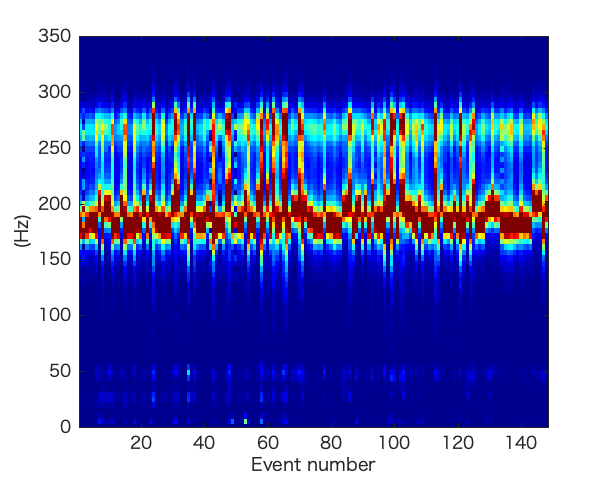
\includegraphics[scale=1] {Flctpspec.png} 
\caption[イベント毎のスペクトル構造: Small fluctuation]
{イベント毎のスペクトル構造: Small fluctuation, Fig. \ref{Monopspec}のキャプションを参照}
\label{Flctpspec}
\end{center}
\end{figure} 


\begin{figure}[H]
\begin{center}
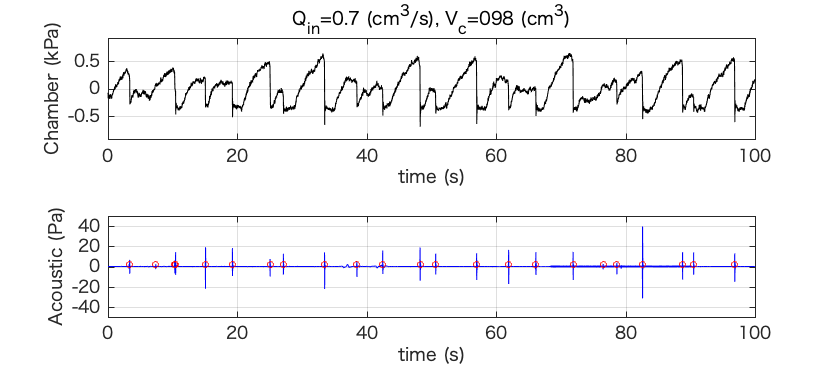
\includegraphics[scale=1] {DistPAtime.png} 
\caption[チャンバー圧力と空気振動: Disturbed STW]
{チャンバー圧力と空気振動: Disturbed STW, Fig. \ref{MonoPAtime}のキャプションを参照}
\label{DistPAtime}
\end{center}
\end{figure} 

\begin{landscape}
\begin{figure}[H]
\begin{center}
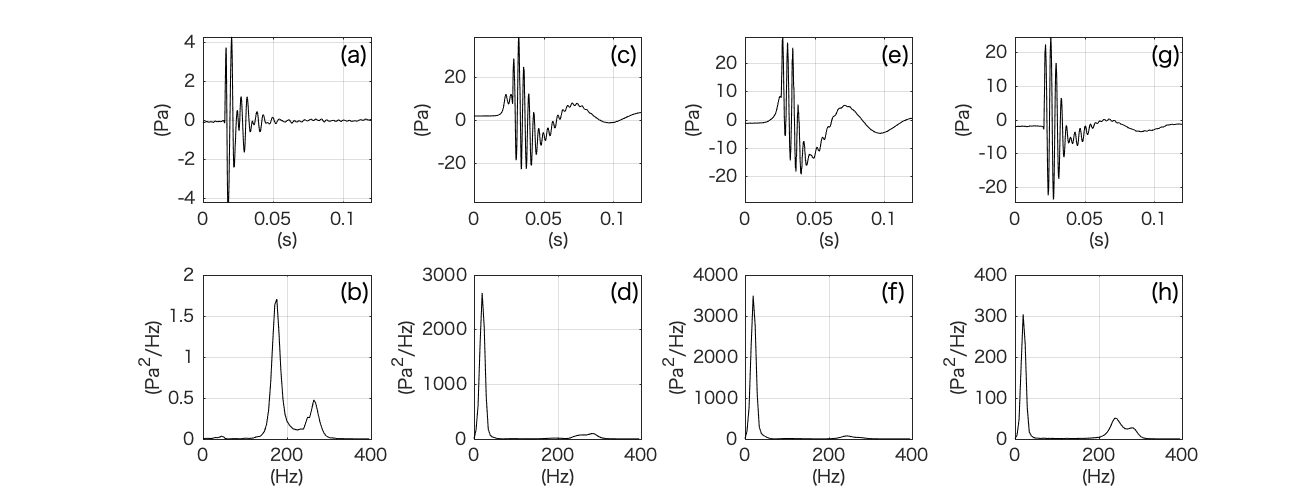
\includegraphics[scale=1] {Distwaveform.png} 
\caption[代表的波形と周波数構造: Disturbed STW]
{代表的波形と周波数構造: Disturbed STW 発生時の代表的波形; (a, b) 高周波パルス, (c-h) 低周波パルス; (c, d) Type 1; (e, f) Type 2; (g, h) Type 3}
\label{Distwaveform}
\end{center}
\end{figure} 
\end{landscape}


\begin{figure}[H]
\begin{center}
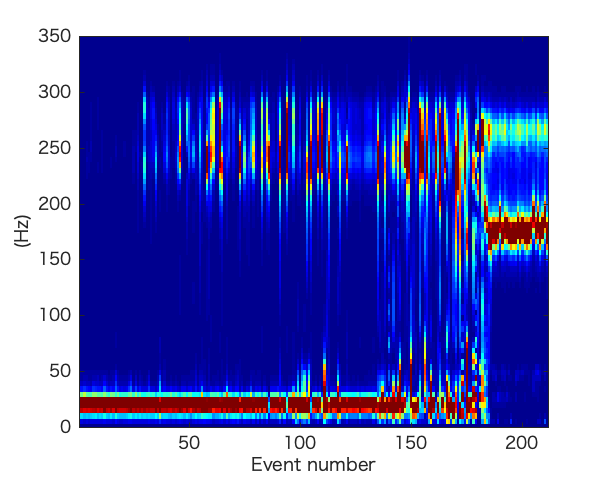
\includegraphics[scale=1] {Distpspec.png} 
\caption[イベント毎のスペクトル構造: Disturbed STW]
{イベント毎のスペクトル構造: Disturbed STW, Fig. \ref{Monopspec}のキャプションを参照}
\label{Distpspec}
\end{center}
\end{figure} 


\begin{figure}[H]
\begin{center}
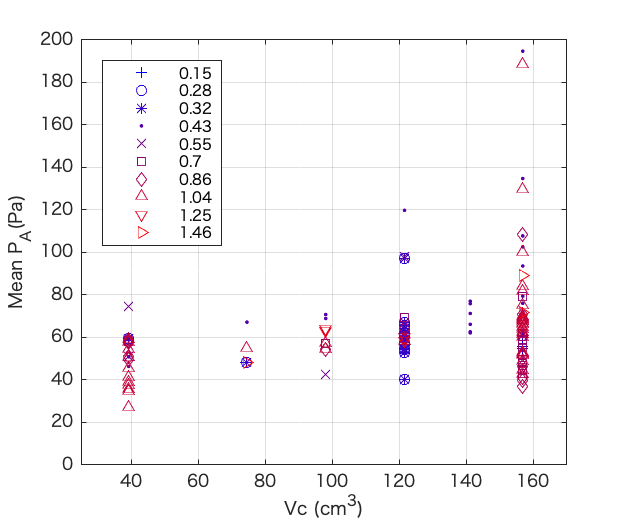
\includegraphics[scale=1] {QVA.png} 
\caption[実験パラメータと空気振動振幅]
{実験パラメータ ($V_\mathrm{c}$, $Q_\mathrm{in}$) と空気振動振幅: マーカーは $Q_\mathrm{in}$ の違いを表す. 凡例の単位は cm$^3$/s.}
\label{QVA}
\end{center}
\end{figure} 






\begin{landscape}
\begin{figure}[H]
\begin{center}
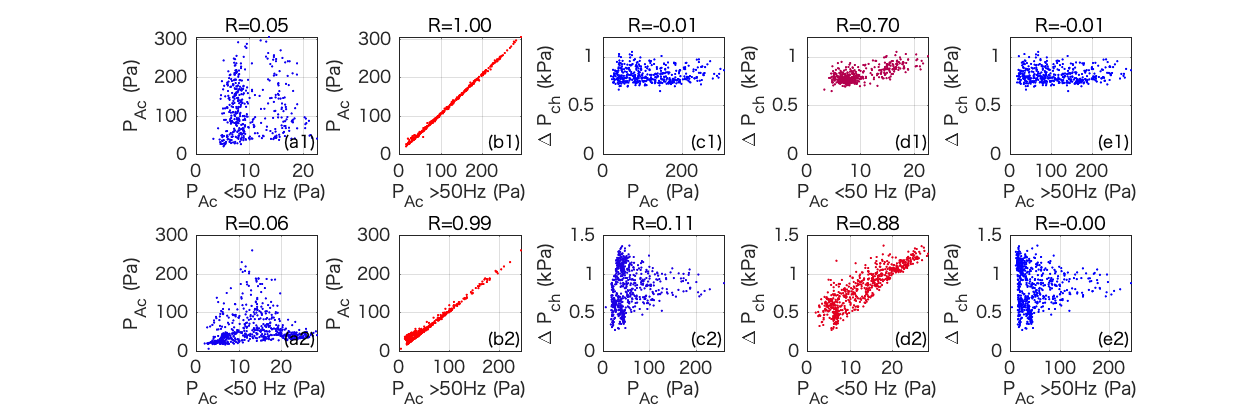
\includegraphics[scale=1] {PAPCall.png} 
\caption[空気振動とチャンバー圧力振幅比較]
{空気振動とチャンバー圧力振幅比較: a1-e1は Unimodal STW, a2-e2は Disturbed STWの結果を示す. 空気振動はチャンバー圧力急減と対応する低周波パルスの振幅を示す. Rはそれぞれのパラメータの相関係数. (a, b) 空気振動生波形振幅 $P_{AC}$と, 空気振動の低周波帯 ( < 50 Hz)振幅 (a), 高周波帯 (> 50 Hz) 振幅 (b). (c, d, e) チャンバー圧力振幅 ($\Delta P_{ch}$) と, 空気振動生波形振幅 ($P_{AC}$, c), 低周波帯振幅 (< 50 Hz, d), 高周波帯振幅 (> 50 Hz, e)の比較}
\label{PAPCall}
\end{center}
\end{figure} 
\end{landscape}




%QVAplot.m 
\clearpage
\subsubsection{パイプ内流れとの比較}
実験で撮影したパイプ内流れ映像, チャンバー圧力変化と, 空気振動パルスの発生を比較する.

STWが発生している時, Fig. \ref{ImPenlarged}によれば, チャンバー圧力の急減圧, すなわち, スラグ-環状流遷移が発生する際の液スラグ膜破裂にともなって, 振幅の大きな (> 10 Pa) 空気振動パルスが発生している. 
この時の波形は Fig. \ref{Monowaveform}d で示した, 低周波パルスである. 低周波パルス発生直後は, パイプ上端からチャンバーまでガス相が一続きになっている.
空気振動波形低周波帯 (< 50 Hz)に, ローパスフィルターをかけた波形と, チャンバー圧力波形を比較する (Fig. \ref{ImPenlarged}). 空気振動低周波帯の波形は, チャンバー圧力減圧時の波形と対応しており, 空気振動低周波帯の増減圧にかかる時間 ($\sim$ 0.05 s) は, チャンバー圧力の減圧にかかる時間と同程度である.

また, チャンバー圧力の急減圧の直前に, Precursor的に, 小さな空振パルスが発生している. この時の小さなパルスは, 全ての液スラグが破裂する直前の, 最上端液スラグ膜破裂に対応しており, Fig. \ref{Monowaveform}a で示した高周波パルスに対応している. この高周波パルスが発生するとき, まだパイプの中にはスラグ流れが存在している. 

Small fluctuation発生時, 準定常的的スラグ流のうち, 最も上端の液スラグ膜が破裂する際に空気振動が発生している. この時, 前章で記述したように, 一番上の膜が破裂しても, 後に続く液スラグ膜は破裂せずそのまま上昇を続けることから, 発生時の状況は, STWにおけるPrecursor的高周波パルスと同じである.

Disturbed STW発生時には, Unimodal STW発生時に比べて, 空気振動波形にバリエーションがある (Fig. \ref{Distwaveform}). そこで, パイプ内流れを高速度撮影 (8000 frame/s) で撮影することで, スラグ-環状流遷移時の液スラグ破裂過程と, 空気振動波形の対応を検討する.

Fig. \ref{Distwaveform}c のような波形 (Type 1) が発生するときのパイプ内流れと空気振動波形の様子を Fig. \ref{Type1} に示す. この波形はUnimodal STWの際に発生する低周波パルス (Fig. \ref{Monowaveform}d) とよく似た波形であり, 高周波と低周波の振動がほぼ同時に始まる. このとき, パイプには液スラグが3つ発生しており, 便宜上, 上からスラグ1, 2, 3とする. この例では, スラグ1が破れた $t=1210$ msに, Precursor的高周波パルスが発生した. 次に, スラグ2と3が 10 ms程度の時間差で破裂したが, その時に高周波と低周波を含む振動が発生したことがわかった.

Fig. \ref{Distwaveform}e のような波形 (Type 2) が発生するときのパイプ内流れと空気振動波形の様子を Fig. \ref{Type2} に示す. 波形は緩やかに立ち上がり, そのままピークに達し, その後高周波の振動が発生する. このような特徴は Unimodal STW発生時にはほとんど見られず, Disturbed STWに特徴的な波形であった. Fig. \ref{Type2} の例では, 液スラグが3つ発生しており, 上からスラグ1, 2, 3とする. スラグ1と3は $t=1650$ msにほぼ同時に破裂するが, この時, まだスラグ2は膜状になるほど薄くなっていない. スラグ1, 3の破裂をきっかけに, スラグ2の上昇速度は大きくなっていき, $t=1720$ ms に破裂する. 破裂前の液膜の変形は, Fig. \ref{Type1} と比べて大きいことから, 緩やかな空気振動の立ち上がりは, スラグ2の破裂直前の変形によるものであると考えられる.

Fig. \ref{Distwaveform}g のような波形 (Type 3) が発生するときのパイプ内流れと空気振動波形の様子を Fig. \ref{Type3} に示す. 空気振動波形は, 液スラグの破裂の直前に, わずかに周期のやや長い増減圧がある. 液スラグ破裂と同時に鋭い立ち上がりに続いて, 高周波振動が始まり, その後低周波振動が続く. パイプ内流れは, パイプ下端で発生した液スラグが, 次の液スラグ再生成の前に液膜流内で破裂している. 高周波パルス (Fig. \ref{Distwaveform}a) と波形が似ているが, この場合, 液スラグ破裂はスラグ-環状流遷移に対応するために, 低周波の振動も発生している.


\clearpage
\subsubsection{空気振動振幅とチャンバー圧力振幅の関係}\label{AcoChp}
 Unimodal STW, Disturbed STW 発生時の空気振動とチャンバー圧力の関係を Fig. \ref{PAPCall} に示す. 空気振動パルスは, スラグ-環状流遷移発生にともなう低周波パルスの振幅と比較する. チャンバー圧力振幅と空振生波形振幅は全く相関がない (Fig. \ref{PAPCall}c). これは, Fig. \ref{MonoPAtime} において, Unimodal STW 発生時にチャンバー圧力が毎サイクルほぼ一定であるにもかかわらず, 空気振動パルスの振幅が一定でないことからもわかる. 低周波パルスは, 低周波帯と (<50 Hz) と高周波帯 (> 50 Hz) にピークを持つことから, それぞれの帯域でローパス, ハイパスフィルターをかけた波形の振幅と, チャンバー圧力を比較する (Fig. \ref{PAPCall}d, e). 低周波パルスの低周波帯ピークとチャンバー圧力に強い相関がある (Fig. \ref{PAPCall}d). Fig. \ref{PAPCall}d1 では チャンバー圧力振幅がほぼ一定であるため, 関係がやや不明瞭であるが, Fig. \ref{PAPCall}d2 ではチャンバー圧力振幅と空気振動低周波帯の振幅に強い相関があることがわかる.

\clearpage
\subsection{議論}\label{ACOdisc}


\subsubsection{空振の特徴的周波数構造}
実験に見られる空気振動は, 低周波パルスと高周波パルスに大別されることが分かった. 管内における膜の破裂によって励起される特徴的な周波数がパイプ内の気柱共鳴である可能性を検討する. パイプ内の膜破裂による空気振動に着目した先行研究 \citep{Vidal2006a, Sanchez2014} では, 特徴的な周波数は閉管の気柱共鳴で説明できるとしていた. 本実験では, パイプの下端はチャンバー側に解放されており, 上端は解放されているため, パイプの構造は両端開口 (開管) になっている. 開管の気柱共鳴の $n$倍振動 ($n=1,2,3...$)の周波数 $f^{op}_{n}$はパイプ長さ $L$, 音速 $c_{air}$を用いて, 以下のように与えられる:
\begin{eqnarray}
f^{op}_{n}=\frac{n}{2L} c_{air}
\end{eqnarray}

高周波パルス発生時には, パイプの途中に液スラグが存在し, 上端のみが開口する, 閉管となっている. 閉管の気柱共鳴の $2n-1$倍振動 ($n=1,2,3...$) 周波数 $f^{cl}_{2n-1}$ は, 閉管部分のパイプ長さ $L_1$として, 
\begin{eqnarray}
f^{cl}_{2n-1}=\frac{2n-1}{4L_1} c_{air}
\end{eqnarray}
と与えられる.

低周波パルスの発生時, パイプの中は連続したガス流れになっていることから, パイプが開管になっている.  また, 低周波パルスの低周波帯の増減圧にかかる時間は, チャンバー急減圧にかかる時間と同程度であった (Fig. \ref{ImPenlarged}). これは, 空気振動低周波帯のシグナルが, チャンバーからのガスの放出によって励起されている可能生を示唆している. そこで, 特徴的な周波数ピークを作る要因として, チャンバー内のガスがバネの役割を果たすパイプ-チャンバー内全体の共鳴, すなわち, ヘルムホルツ共鳴が考えられる.

ヘルムホルツ共鳴によって励起される周波数 $f_h$は, パイプの断面積 $S$ とした時, チャンバー体積 $V_\mathrm{c}$ を用いて,  
\begin{eqnarray}
f_{h}=\frac{c_{air}}{4\pi} \sqrt{  \frac{S}{V_\mathrm{c} L }   } \label{Helmeq}
\end{eqnarray}
と与えられる. 

Fig. \ref{Helm}に, パイプ全長 630 mm, パイプ内径 2.5 (1.8) mm, 音速 340 m/sとした時の, ヘルムホルツ共鳴および気柱共鳴によって励起される基本周波数を示す. 

低周波パルスにおいて, 発生する低周波ピークは, パイプ半径が 1.8 mm の時のヘルムホルツ共鳴の周波数ピークとほぼ一致している. 装置のパイプ半径は 2.5 mm であるが, 液膜流が存在しているため, 実効的なガス流路半径が小さくなっていると考えられる. 

また, 低周波パルスは高周波帯 (230 - 270 Hz) にもピークを持っていた. これは, 630 - 700 mm の開管パイプの気柱共鳴基本周波数に相当し, 実験パイプの全長 630 mmと整合的である. 

高周波パルスのピークはやや低い周波数で, 180 - 200 Hz 付近にピークを持っていた, これは, 430 - 460 mm の閉管パイプの基本周波数に相当するが, 液スラグはパイプ下端から 200 mm 程度のところで破裂するという実験での観察結果と整合的な値である. ただし, どちらのパルスも倍音構造は基本周波数の整数倍からずれており (Fig. \ref{Monowaveform}), 液スラグの存在や, 液膜流によるパイプ内の構造を含めて今後さらに検討が必要である.

以上の考察から, 実験にみられる空気振動は, 低周波帯と高周波帯にピークを持っており, 低周波帯はパイプ-チャンバー全体の構造を反映したヘルムホルツ共鳴, 高周波帯はパイプの構造を反映した気柱共鳴の基本周波数によって説明できると考えられる.



\subsubsection{空振の特徴的波形}
Unimodal STWと, Disturbed STWでは, スラグ-環状流遷移発生にともなう低周波パルスの波形の特徴が異なっていた. これは, \S \ref{preflowanalysis}でも指摘したように, Disturbed STWにおける液膜流厚み及び液スラグ上昇速度のばらつきに起因していると考えられる. これについて, 考察を進める.

Unimodal STWが発生しているとき, 液膜流の厚みにはほとんどばらつきがなかった (Fig. \ref{RDKhist}). このため, 液スラグの上昇の仕方も各STWサイクルでほとんど変わらない. 高周波パルスは最上部の液スラグだけが先行して破裂することによって発生しており, Fig. \ref{Monopspec} によれば, 高周波パルスと低周波パルスはほぼ同数であった. このことから, Unimodal STWでは, スラグ-環状流遷移過程も毎サイクルほとんど変わらず, 毎回最上部の液スラグが先行して割れて高周波パルスを発生し, それに続いてパイプ内の液スラグがほぼ一斉に (10 ms以内) に破裂して低周波パルスを発生していると考えられる.

Disturbed STWでは, 液膜流途中で液スラグ再生成が発生することによって, 液スラグの上昇速度にばらつきが生じ, 結果として液膜流厚みにもばらつきが生じていた (Fig. \ref{RDKhist}). このことで, スラグ-環状流遷移時の液スラグ膜破裂過程もばらつき, 様々な空気振動波形が計測されていると考えられる. Fig. \ref{Distpspec} によれば, Unimodal STW発生時に比べて, Disturbed STWでは, 高周波パルスの割合が少ない. これは, スラグ-環状流遷移の際に, 複数液スラグのうち, 必ずしも最上部の液スラグから割れ始めるのではなく, 下部の液スラグから破裂する, または, 複数の液スラグが再生成する前に液スラグが破裂するといった異なるスラグ-環状流遷移過程も含んでいることを反映している.
特に, Fig. \ref{Type2} の空気振動波形に対応する破裂直前に, 液スラグ急速に加速するような時には, それだけ多くの液を液膜流に排出し, 大きな液膜流表面擾乱を発生させると考えられる. 大きな液膜流表面擾乱が発生すれば, 液膜流途中での液スラグ再生成が発生しやすくなり, Disturbed STWのような周期の乱れを生み出すと考えられる (\S \ref{precond}). 

%しかし, 一方で空振波形とSTW継続時間に明瞭な定量的関係を見出すことはできなかった. 今後, 液膜の変形過程や速度, 液膜流の関係を詳細に調べる必要があると考えているが, 本研究ではこれ以上議論しない.

\subsubsection{空振各帯域振幅, チャンバー圧力振幅の関係}

%生波形振幅は高周波帯振幅と問い相関を持つことから, 生波形の振幅は管内の気柱共鳴音を表していることが示唆されが, 一方で, チャンバー圧力振幅と, 空気振動生波形振幅はほぼ相関が見られない. これは, \cite{Vidal2006a} が指摘するように, 気柱共鳴音の振幅は, 膜の破裂速度に強く依存することが一つの要因であると考えられる. 膜の破裂速度を推定するためにはさらに高速度のビデオ撮影が必要であるが, これは本実験の測定範囲外であるため, これ以上の議論は行わない. 

空気振動波形のうち, ヘルムホルツ共鳴に起因する低周波帯空気振動の振幅は, チャンバー圧力振幅と良い相関を示した. Fig. \ref{AcoAmVP} では, STWが発生するすべての実験条件において, 空気振動低周波帯の振幅 (縦軸) と, チャンバー圧力振幅, チャンバー圧力振幅とチャンバー体積の積 (噴出ガス量に相当) を比較した結果である. この結果によれば, 空気振動低周波帯の振幅は, チャンバーの圧力振幅, すなわちスラグ-環状流遷移直前のチャンバー過剰圧と良い比例関係にある. 一方で, チャンバーの体積 ($V_\mathrm{c}$) の情報がなければ, 噴出ガス量の推定ができないことも示している. 

Eq. (\ref{Helmeq}) によれば, パイプの構造 ($S$, $L$) と音速が既知でない限り, 低周波帯のピーク周波数  ($f_{h}$)  から $V_\mathrm{c}$ を見積もることも難しい. 一方で, 音速さえ既知であれば, 低周波パルスに含まれる高周波帯のピーク周波数 ($f^{cl}_{1}$) から, $L$ を推定することができる. 例えば, パイプの中が見えない場合でも, $S$ の値として, 表面で観察できるパイプ上端のガス流路断面積を用いれば, Eq. (\ref{Helmeq}) を用いて $V_\mathrm{c}$ を推定できる. 
ただし, 実験の結果 (Fig. \ref{Helm})によれば, $S$ の値として液膜流の存在よって実際のパイプ断面積よりも小さいガス流路断面積を用いた方が, 実験パラメータ $V_\mathrm{c}$ をより説明することができた. すなわち, $S$ の値としてパイプの断面をそのまま用いると, チャンバー体積を過大評価してしまう可能性には注意が必要である.


\clearpage
\subsubsection{火山学的示唆}\label{acoshisa}
実験の結果からは, 空気振動波形の違いによるチャンバー圧力振動周期への影響を定量的には議論できなかったが, チャンバー圧力振動周期が乱れるような時に, 空気振動波形にバリエーションがある, ということを実験の解析から示した.
Disturbed STW発生時に見られた, Fig. \ref{Type2} の空振波形では, 高周波振動に先行して, 緩やかな波形の立ち上がりが見られた. このような先行相は, ブルカノ式噴火にともなった観測例が報告されている. \cite{Yokoo2009}では, 空振波形とビデオ映像を合わせて, 爆発の主要相に先行する空振記録の緩やかな増圧は, 爆発直前の火口直下ガスポケットの膨張による, 浅部プラグの変形に起因していると推定している. 実験の結果を基にすれば, このようなプラグの破壊にともなう火口浅部構造の変化や, 噴出物の再堆積等が, 噴火の周期に影響を及ぼしているかもしれない (\S \ref{sugvolc}). 


もう一つ, この実験から得られた重要な知見は, 空振のある特徴に着目すれば, 地下の圧力源圧力変化にともなう地盤変動といった地下の情報を含んでいる可能性がある, という点にある.
実験では, 空振低周波帯のシグナルと, チャンバー減圧が同程度のタイムスケールであり (Fig. \ref{ImPenlarged}), このタイムスケールに相当する低周波帯の空気振動振幅と, チャンバー圧力振幅に対応関係があった. この結果を踏まえると, 実際の観測においても, 地盤変動と同程度のタイムスケールの空振シグナルに着目すれば, 地盤変動と空振の対応関係を見い出すことができるのではないかと考える.
先行研究において, 火山活動にともなって発生する空振と噴出量や噴出率の関係は様々なメカニズムが提案されており, 統一的な理解は進んでいないが, 特定のメカニズムに着目すれば, 噴出量・噴出率といった情報との対応関係を見いだせる可能性があると指摘されている \citep{Ichihara2016a}.

実験では特定の周波数ピークを含む空気振動周波数帯の振幅と, チャンバー圧力振幅を比較した. 火山噴火にともなう空振にも, 特徴的な周波数ピークがあることが先行研究で報告されている \citep{yokoo2012bo}. 実験との対比として, 火山活動にともなって発生する空振において, ある特定の周波数帯が, 地盤変動といった地下の情報との対応関係を検討する必要があると考える.

先行研究では, 爆発にともなうパルス状の空振波形に着目し, 積算体積を推定する手法が提案されており \citep{Johnson2003}, 例えば, 桜島昭和火口活動にともなった空振記録と, 火山灰噴出量との比較が試みられている \citep{Fee2017a}. しかし一方で, 例えば桜島における爆発的噴火にともなう地盤変動の継続時間は, 数分から数十分であり \citep{Iguchi2012, Iguchi2013a}, 爆発パルスの継続時間は数十秒である.
\cite{DelleDonne2016} では, Ash-richな噴火においては, 爆発の初動パルスだけではなく, 後続相にも注目することで, 噴火にともなって放出される熱エネルギーと良い相関が得られること指摘している. 本実験の結果を踏まえれば, 地盤変動との対応関係を検討するためには, 爆発にともなう初動パルスだけに着目するではなく, それに続く後続波まで含めた空振シグナルとの継続時間や物理量の対応関係を検討する余地があると考える. パルス的な空振だけに注目するのではなく, 継続時間の長い後続相にまで着目することで, 地盤変動に対応するような地下の情報を含んでいる可能性があることが本実験から示唆されると考えられる.



%bibliography作成にはMendeleyを用いた
%Mendeleyを用いてbibファイルをこのtexファイルと同じディレクトリ内に作成. ターミナル上で " pbibtex ファイル名" を実行してコンパイル
%http://pioneerboy.hatenablog.com/entry/2014/01/18/214446
%http://ftp.yz.yamagata-u.ac.jp/pub/CTAN/macros/latex/contrib/natbib/natbib.pdf
%Agu08.bst をどこから入手したのかわすれてしまった...
%agu_template内
\clearpage \newpage
\bibliographystyle{agu08}
\bibliography{library} 
\addcontentsline{toc}{section}{References}


\end{document}